\chapter{Background}
\label{ch:background}
Introduction

Parallel programs have been common in scientific analyses as a mean to improve performance or to handle large scales of data. Currently, it is being adopted into other domains as well with the rising data sizes and the availability of computing power in bulk. The steps of forming a parallel program [5] are given in Figure 1.
 
\begin{figure}
\centering
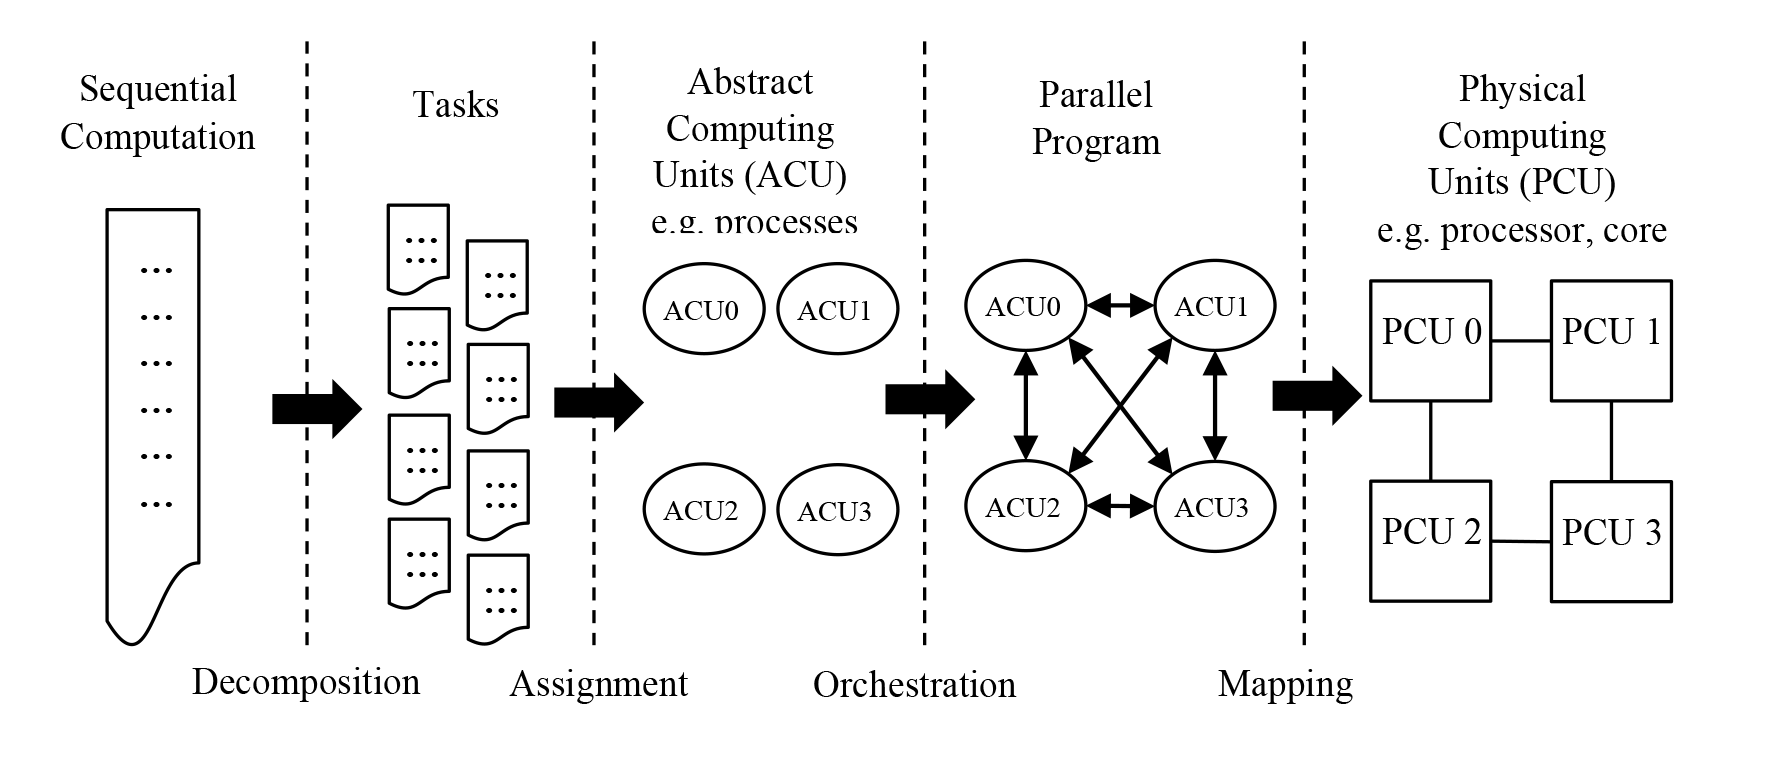
\includegraphics[width=0.9\columnwidth]{figures/fig_parallel_decompose}
\caption{Steps of creating a parallel program}
\label{fig:fig_parallel_decompose}
\end{figure}

Decomposition generally means to decompose the domain where computations for sub domains may be done in parallel with data exchanged at boundaries. This technique is known as data parallelism in the literature [10]  and is not be confused with the idea of pleasingly parallel applications. In data parallelism the computations on sub domains will be similar to each other. Another form of parallelism that one could exploit in decomposition stage is task parallelism [10] where non interdependent different computations are run in parallel. 
Once the decomposed tasks are identified, they need to be assigned to abstract computing units (ACU) in the particular parallel programming language or library (hence-forth distinguished from the term “language” only if necessary). Parallel languages provide constructs to create ACUs in one or more of the following forms.

	Explicit Parallel Constructs
In this form the programmer explicitly instructs the runtime to execute a designated segment of code in parallel. Spawning a new process using the classical fork system call, start() method in java.lang.Thread class, Parallel.Foreach in Microsoft Task Parallel Library (TPL), and forall in Chapel are example constructs of this form.
	Implicit Parallelization
	This is compiler introduced parallelization for known patterns of code without affecting the semantics of the program. For example, Fortress evaluates segments like tuples, for loops, also do blocks, and function arguments in parallel.
	Compiler Directives
	This may be considered as both explicit and implicit forms of parallelization since the programmer explicitly inform the segment to be parallelized while compiler performs the breakdown of it in to parallel tasks. For example, the \#pragma omp parallel for directive in a C or C++ program based on OpenMP informs the compiler to generate library calls to parallelize the for loop following the directive.
    
To avoid any confusion, we would like to emphasize 3here that ACUs do not need to be fixed at start time or execute the same code in a single program multiple data (SPMD) fashion.
Decomposition may result in dependencies, which needs to be handled through some form of communication between ACUs. This may not necessarily be through message passing between ACUs. Globally shared data structures could be used in orchestration as well. In fact, the model of orchestration is specific to the programming model of the language where some may provide fully-fledged communication between ACUs while some may restrict to specific patterns only. The original MapReduce model [6]  for example, allows communication between Map and Reduce tasks only. However, it is also worth noting that complex parallel applications may even be developed over less sophisticated programming models. Parallel implementations of latent Dirichlet allocation (LDA) [15] and deterministic annealing multi-dimensional reduction [2] for example are some non-trivial applications developed on the restricted MapReduce model.
The parallel program development is complete after orchestration. The remaining step is to map ACUs to physical computing units (PCU), which is done by the language’s runtime. Note the user may have some control over the mapping such as specifying the maximum number of cores to use, etc. but most of the control is up to the runtime. 
Parallel Programming Memory Models
One classifier of parallel languages is the memory model, which we intended to identify the abstraction of the address space of a program rather the physical composition of memory hence-forth. In fact, the models discussed below may be implemented on either physically shared or distributed memory systems [10]. Three major memory models are being used at present as described in the following sections.
Shared Memory Model
This model presents the programmer with a shared memory layer to his or her programs. The programmer’s view of the program is then a collection of tasks acting on top of a single address space as shown in Figure 2.
 
\begin{figure}
\centering
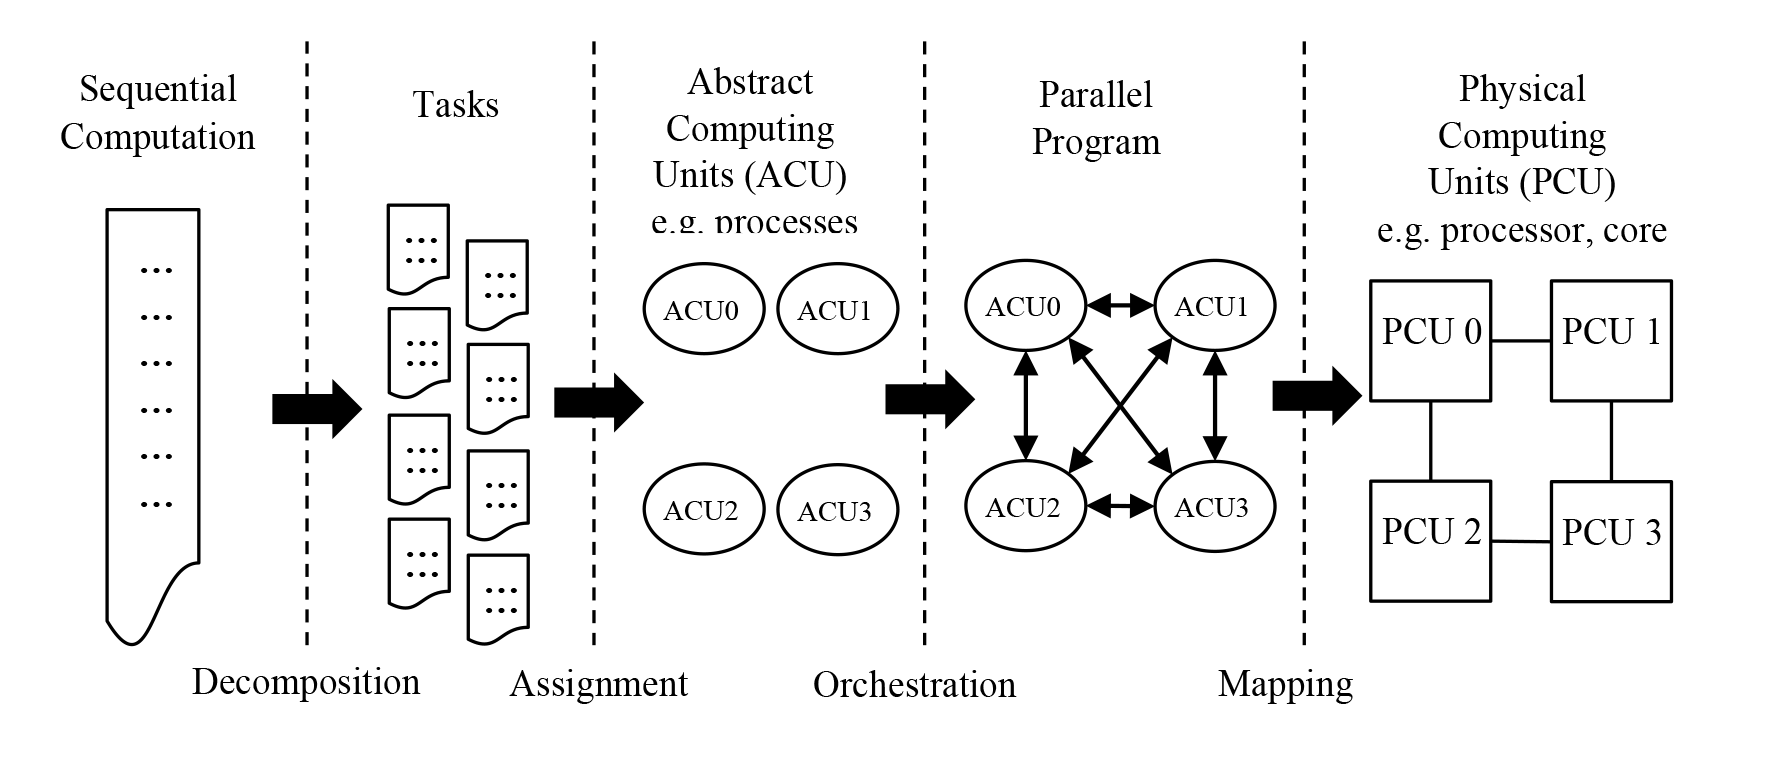
\includegraphics[width=0.9\columnwidth]{figures/fig_parallel_decompose}
\caption{Programmer’s view of a shared memory model}
\label{fig:fig_parallel_decompose}
\end{figure}


The language supporting a shared memory model is responsible for mapping it on to the physical computing system. Usually a task will get mapped to an executable entity in the operating system like a Light Weight Process (LWP). Note. The mapping may not necessarily be one to one and may even take the forms of one to many and many to many. Implementing the shared view of global address space with physically distributed memory is not straightforward and requires communication. Overall the architecture of a shared memory model implementation would be similar to Figure 3. Note. The leftmost processor is enlarged to show the mapping of tasks into central processing units (CPU), and the network layer is depicted between processor and memory of each machine for the sake of clarity and does not imply uniform memory access. Also, though not shown in the figure, tasks can have unshared local address spaces in physical memory local to the processor running the particular task.
 
Figure 3. Architecture of shared memory model implementation
Access of a variable that is global to tasks requires transfer of data via network from the residing machine’s memory to the requested task. This transfer is made transparent to the programmer by the programming language. Implementations may take the advantage of physically shared memory if exist and may even refrain from supporting distributed memory systems. It is natural in such cases to combine this model with another model supporting distributed memory systems, which coincidently fits well with present day multi-core nodes.
The highlight of this model in a programmer’s perspective is the ability to share data among tasks without being constrained by the notion of ownership, which would otherwise result in explicit communication to share data. This property is identified as global view of computing, which is presented in section 3.2. The caveat, however, is the need to synchronize data accesses to preserve the expected behavior of the program. 
Open Multi-Processing (OpenMP)
OpenMP is one of most popular implementations of shared memory models. It provides an Application Programming Interface (API) based on compiler directives to express parallelism explicitly and a set of library routines and environment variables. Realizations of this standard supports C/C++ or Fortran languages and portable enough to run on both Unix/Linux and Windows based platforms. OpenMP may not be used directly on distributed memory architectures as it supports only shared memory systems.
An OpenMP program by default follows a fork-join execution model in which a master thread starts at the entry point and threads are forked to execute the denoted parallel regions followed by a join of the threads as depicted in Figure 4.
The number of threads spawned in the parallel region may be decided by the programmer by setting OpenMP execution to static mode and specifying it manually in which case the program is either guaranteed to get that many threads for each parallel region or fail otherwise. The decision on the number of threads may either be left to the operating system by turning on the dynamic execution mode and specifying the maximum number of threads to use if possible, though it may use less than that. In either case, all the threads are numbered from zero to one less than the total number of threads. Thus, it is also possible for different threads to take different paths of executions depending on their thread number inside a parallel region. Finally, OpenMP gives several synchronization constructs, i.e. critical, atomic, barrier, master, ordered, and flush, to the programmer to avoid race conditions when multiple threads work on shared data.
POSIX Threads (Pthreads)
Pthreads is a different yet equally popular implementation of this model. It is a user level library supporting the notion of threads for C programs. Unlike OpenMP, the programmer needs to explicitly encapsulate the code to be run in parallel by a thread. A Pthread program is a single process with threads being spawned along its execution time as intended by the programmer. Threads are separate sequences of execution with no notion of a hierarchy, i.e. parent-child relationship, and dependency between them. Typical execution model of a Pthread program is show in Figure 5.
The program starts with a single thread, T1. It continues execution for some time and spawns T2 and T3. All T1, T2, and T3 continue to execute until T1 terminates. T2 and T3 continue and spawn more threads down the line. Each horizontal line near the arrow heads indicates the termination of the particular thread, hence the entire program terminates at the end of T4 according to the diagram. 
Joining threads similar to the case with OpenMP is also possible with Pthreads. The pthread_join construct, which does this, blocks the calling thread until the other, i.e. joining, thread specified by a thread-id terminates. However, it is an error to attempt multiple joins on the same joining thread.  Pthreads also supports two other thread synchronization mechanisms called mutexes and conditional variables. In depth details on these, however, are not in the scope of this paper.

 
Figure 4. Fork-join execution model of OpenMP

Figure 5. Execution model of a Pthread program
Distributed Memory Model
Distributed memory model, as it name suggests presents a segmented address space where each portion is local only to a single task. The programmer’s view of the program is a collection of individual tasks acting on their own local address spaces as shown in Figure 6. Programmer's view of distributed memory model
 
Figure 6. Programmer's view of distributed memory model
In contrast to the view of a program based on shared memory model as shown in Figure 2, this presents a share nothing view in terms of address space of the program. This obligates the programmer to partition data structures that need to be distributed among tasks manually. In essence, this model does not support the notion of distributed data structures. Another implication is that tasks need a mechanism to communicate between each other to cooperatively work in parallel as shown in dashed arrows in Figure 6. 
The share nothing view also encourages a SPMD programming model. Unlike in shared memory model implementations where a single thread starts the execution, multiple tasks start executing the same program independently with SPMD. A task id assigned by the underlying implementation is used to differentiate the flow of execution inside the program. 
Mapping of this model on to the physical hardware is fairly straightforward where a task would get mapped to a unit of execution in the operating system as before and the address space local to the particular task would get allocated in the physical memory local to the processor running the task. Figure 7 depicts an overview of the mapping of this model onto physical hardware. The leftmost processor and memory are enlarged to show the mapping of tasks and address spaces.
Accessing data remote to a particular task requires explicit communication over the network as indicated in Figure 7. The programmer is responsible for using the constructs provided by the underlying abstraction to specify such communication. Variables local to a task reside in physical memory of the same machine and require no network communication to access them. 

 
Figure 7. Architecture of distributed memory model implementation
Accessing memory nearer to a CPU is always faster than accessing remote or far away memory in computer systems. The per task memory abstraction thus naturally overlays with this property in hardware, thereby giving the benefit of improved performance through data locality to the programs. The main disadvantage of this abstraction is the local (fragmented) view of computing and the need to express communication explicitly. Section 3.1 presents the local view of computing in detail.
Hybrid Approach
It has been common to combine shared memory model implementations such as OpenMP or Pthreads with a distributed memory model implementation such as MPI for inter-core parallelism while keeping MPI as the mean for inter-node parallelism. The view of a program with this hybrid approach is shown in Figure 8.
 
Figure 8. Programmer's view of the hybrid approach

There are two types of tasks visible in Figure 8, i.e. inter-node tasks and inter-core tasks, which are represented in large ellipses and small ellipses respectively. In practice, these may be MPI processes and Pthread or OpenMP threads. Each inter-node task is assigned with a local address space as in Figure 6, yet a portion of this is used by inter-core tasks as the shared address space among them. Total parallelism achievable in this setting is equal to the product of inter-node tasks and inter-core tasks. Also, in a multi-core environment where cores share physical memory, this approach seem to work efficiently than having pure MPI processes equal in parallelism.
 Message Passing Interface (MPI)
MPI is an API specification allowing inter-process communication via message passing. Over the years it has become a de facto standard in communication among processes and is used by programmers commonly in realizing the distributed memory model. Implementations of the MPI specification are available for several languages like C, C++, and Fortran. Language bindings are available for some other high-level languages like Perl, Python, Ruby, and Java. Also two implementations are available for .NET based languages, i.e. Pure Mpi.NET and MPI.NET.
The execution of an MPI program requires specifying the total number of processes ahead of time. This number indicates the total parallelism of the solution and is fixed throughout the execution of the program. This constraint of fixed number of processes is relaxed in the set of MPI-2 extensions introduced over the original MPI-1 specification allowing an application to create and terminate processes after being started. 
The typical execution model of an MPI program with a fixed number of N processes is depicted in Figure 9 where each MPI process is ranked from 0 to N-1.
 
Figure 9: Execution model of an MPI program
Although not restricted, the usual practice with MPI is to execute the same program code by all the processes resembling the SPMD model of execution. The flow of execution, however, may differ across processes as instructed in the program code based on the rank. This is illustrated in Figure 9 by dashed lines in the flow of execution. Also, these processes operate on separate data entities since there is no notion of distributed data structures. Thus, data sharing is made explicit through communication between processes as indicated by non-vertical arrows. MPI also supports patterns such as two-sided send and receive, broadcasts, reductions, and all-to-all. 
MPI, though supports a fragmented view of computing, has been successful greatly as a mean of implementing parallel programs. MPI’s success is credited for its six properties, i.e. portability, performance, simplicity and symmetry, modularity, composability, and completeness [7]. It is fair to mention that portability, performance, and completeness have attracted the scientific community towards MPI though other properties are equally important. The three properties are briefly discussed below.
Typical lifespan of parallel applications exceeds that of the hardware since high performance computing (HPC) systems tend to evolve rapidly. Thus, having an API like MPI, which does not require the knowledge of the target platform, makes programs easily portable across different hardware architectures. 
The natural match of MPI’s programming model and memory locality yields good performance values for MPI programs. Also, MPI being a library makes it possible to get the advantage of the best compilers available. MPI, however, is not able to give the best performance for a single source across different target platforms even though it supports both portability and performance. This lacking feature is defined as performance portability and realistically it is an unsolved problem even for Fortran on uniprocessor systems.
Finally, MPI is a complete programming model meaning that any parallel algorithm can be implemented with MPI, though it may not be easy. It has 128 routines in MPI-1 and 194 routines in MPI-2, to support such a general case of parallel programming problems. Unfortunately though, this rich collection of routines is often mistaken as an unnecessary complexity of the framework.
Partitioned Global Address Space (PGAS) Model
PGAS model tries to incorporate the best of both shared and distributed memory models, namely, simple data referencing and programmability of the former and data locality of the latter. It does so by providing a global address space, which is partitioned to make the tasks acting upon it aware of the locality. The programmer’s view of the program with this model resembles a superimposed view of Figure 2 and Figure 6 as presented in Figure 10. 

 
Figure 10. Programmer's view of a PGAS model

Each task has a private address space similar to the case with distributed memory model. Also, a portion of the total address space allocated for a task contributes to the shared space among tasks as well. The shared space in this model, however, enables a programmer to get the advantage of data affinity since there is a notion of partitions as shown by dashed vertical lines in Figure 9. This is different from the address space of shared memory model in Figure 2 where there was no ownership for global variables. Also, the presence of a shared address space removes the explicit communication exhibited in Figure 6 and Figure 8 for sharing data. Another importance difference, though not visible from Figure 10, is how implementations support the separation of shared and local variables. Unlike the usual lexically global shared-ness in shared memory model implementations, the PGAS languages explicitly differentiate global and local variables statically. For example, the variable allocation of a simple case is shown in Figure 11.
The array in Figure 11 brings out another feature that was not present with the distributed memory model, i.e. distributed data structures. The distribution of elements in the array may take either a round-robin, block-cyclic or other custom form supported by the implementation. In general, languages with a PGAS memory model may extend the support for distributed data structures beyond arrays as presented in a latter part of this paper. 
Mapping of the PGAS model on to HPC hardware may be achieved with architecture similar to Figure 7 except the implementation is required to introduce necessary communication to refer remote memory. This is an advantage over the case where communication is made explicit by the programmer. Thus PGAS languages can support a cleaner syntax for remote data access.
PGAS, similar to distributed memory model, starts off a program with a fixed number of execution units or threads. These threads work independently executing the program in an SMPD fashion. The model thus follows a local view as explained in section 3.1, though the presence of distributed data structures greatly reduces burden of data access. Also, the threads may exploit the locality of shared data to achieve better performance.
 
Figure 11. Variable allocation of a sample PGAS program


